\documentclass[11pt]{article}
\usepackage{outline}
\usepackage{pmgraph}
\usepackage{listings}
\usepackage{pdfpages}
\usepackage{rotating}
\usepackage{graphicx}
\usepackage{lscape}
\usepackage{subcaption}
\usepackage[normalem]{ulem}
\title{\textbf{Heuristic Optimization Techniques }\\Exercise 3}
\author{David Fankhauser, 1025876\\ Christoph Weiler 1029175\\Gruppe 1}
\date{\today}
%--------------------Make usable space all of page
\setlength{\oddsidemargin}{0in}
\setlength{\evensidemargin}{0in}
\setlength{\topmargin}{0in}
\setlength{\headsep}{-.25in}
\setlength{\textwidth}{6.5in}
\setlength{\textheight}{8.5in}
%--------------------Indention
\setlength{\parindent}{1cm}

\begin{document}
\lstset{language=C++}
%--------------------Title Page
\maketitle
 
%--------------------Begin Outline
\section{Advanced Local Search Description}
We implemented a \textit{General Variable Neighbourhood Search} based on our four neighbourhoods from assignment 2, namely Ordering 1-Shift (\textit{sho}), Shift Edges (\textit{moe}), 
Max-Crossing Neighbourhood (\textit{map}) and Min-Max-Crossing Ordering (\textit{mmc}).
For a neighbourhood description see report-2.

Our previous approach of computing the number of crossings was rather inefficient: To create a neighbour, we copied the old solution, made a change to generate a new neighbour and finally used delta evaluation to compute the number of crossings in a fast way.
However, generating a neighbour by copying a solution is computational expensive. Hence, we only copy solutions, if a better neighbour was found which increased the performance by roughly $4$ times.

In that way we were able to run Variable Neighbourhood Searches in the given time frame.

From theory we expected varying results, when using different orders for the same neighbourhoods.
We were able to confirm this statement empirically.
On each instance we experienced the best results when using a neighbourhood that shifts edges to another page and then improving the ordering (See Appendix for a graphical view).

\section{Experimental Setup}
We tested our program on our local computer because in this assignment we used cmake for cross-platform development and the boost library.
The needed tools were not installed on Eowyn nor Behemoth therefore we decided to test our application on our computers.
The test environment for the results are a Intel Core i7-2600K processor on Ubuntu 15.10.
Our code is written in C++11 and it was compiled with gcc 5.2.1.

\newpage
\section{Results}
For the evaluation we use the following keys:
\begin{itemize}
	\item g = greedy construction heuristic
	\item sho = shift ordering neighbourhood
	\item moe = move edge neighbourhood
	\item map = Max crossing page neighbourhood
	\item mmc = Min-Max crossing ordering neighbourhood 
	\item f = first-improvement step function
	\item r = random step function
	\item vns = Variable Neighbourhood Search
\end{itemize}
\subsection{Results of VNS applied with two neighbourhoods}
{
\center
\begin{tabular}{c|rr|rr}
                 & \multicolumn{2}{c}{g+vns[sho+f,moe+f]}   & \multicolumn{2}{c}{g+vns[mmc+f,map+f]}  \\
Instance         & Obj     & Time                & Obj     & Time               \\
\hline
automatic-1.txt  & 9       & 4.35 ms             & 19      & 6.99 ms            \\
automatic-2.txt  & 0       & 14.18 ms            & 3       & 23.29 ms           \\
automatic-3.txt  & 49      & 100.55 ms           & 78      & 40.93 ms           \\
automatic-4.txt  & 7       & 154.01 ms           & 36      & 8.42 ms            \\
automatic-5.txt  & 10      & 109.48 ms           & 12      & 22.82 ms           \\
automatic-6.txt  & 7456783 & 900000.00 ms        & 6327391 & 175168.00 ms       \\
automatic-7.txt  & 21999   & 900000.00 ms        & 23545   & 5587.51 ms         \\
automatic-8.txt  & 596130  & 900000.00 ms        & 402355  & 181285.00 ms       \\
automatic-9.txt  & 814918  & 900000.00 ms        & 601204  & 900000.00 ms       \\
automatic-10.txt & 28523   & 900000.00 ms        & 27215   & 27286.30 ms        \\
\end{tabular}
}

\subsection{Results of VNS with all neighbourhoods with randomized step functions}
{
A VNS search on the instances 6-10 is still quite exhaustive.
Therefore we treat these instances seperately with a lower number of runs.
\center
\begin{tabular}{c|rrrrrrr}
                & \multicolumn{6}{c}{g+vns[mmc+r,map+r,sho+r,moe+r]}                   \\
Instance        & Best Obj & Mean Obj & Std Dev Obj & Mean Time  & Std Dev Time & Runs \\
\hline
automatic-1.txt & 9        & 11.32    & 1.61        & 621.60 ms  & 85.31 ms     & 50 \\
automatic-2.txt & 0        & 0.26     & 0.66        & 1478.52 ms & 122.67 ms    & 50 \\
automatic-3.txt & 42       & 48.74    & 3.35        & 6015.53 ms & 936.27 ms    & 50 \\
automatic-4.txt & 0        & 2.60     & 1.89        & 3216.76 ms & 364.00 ms    & 50 \\
automatic-5.txt & 2        & 4.64     & 1.35        & 3503.22 ms & 369.22 ms    & 50 \\
\end{tabular}

\begin{tabular}{c|rrrrrrr}
                & \multicolumn{6}{c}{g+vns[map+r,mmc+r,moe+r,sho+r]}                   \\
Instance        & Best Obj & Mean Obj & Std Dev Obj & Mean Time  & Std Dev Time & Runs \\
\hline
automatic-1.txt & 9        & 12.06    & 1.26        & 597.11 ms  & 74.62 ms     & 50 \\
automatic-2.txt & 0        & 0.34     & 0.68        & 1492.39 ms & 142.34 ms    & 50 \\
automatic-3.txt & 40       & 50.80    & 3.36        & 4819.61 ms & 686.03 ms    & 50 \\
automatic-4.txt & 0        & 3.80     & 2.16        & 3660.42 ms & 506.85 ms    & 50 \\
automatic-5.txt & 3        & 4.82     & 1.19        & 3336.54 ms & 428.98 ms    & 50 \\
\end{tabular}

\vspace{0.5cm}

\begin{tabular}{c|rrrrrrr}
                 & \multicolumn{6}{c}{g+vns[mmc+r,map+r]}                   \\
Instance         & Best Obj & Mean Obj   & Std Dev Obj & Mean Time    & Std Dev Time & Runs \\
\hline
automatic-6.txt  & 2092733  & 2194286.00 & 138977.55   & 900000.00 ms & 0.00 ms      & 3 \\
automatic-7.txt  & 24235    & 24578.00   & 246.73      & 34735.63 ms  & 7540.72 ms   & 3 \\
automatic-8.txt  & 392710   & 394370.33  & 1225.99     & 487229.67 ms & 57619.84 ms  & 3 \\
automatic-9.txt  & 643847   & 671164.33  & 19356.36    & 849122.67 ms & 35975.91 ms  & 3 \\
automatic-10.txt & 26732    & 26795.67   & 59.42       & 268704.67 ms & 28534.18 ms  & 3 \\
\end{tabular}

\vspace{0.5cm}

\begin{tabular}{c|rrrrrrr}
                 & \multicolumn{6}{c}{g+vns[map+r,mmc+r,moe+r,sho+r]}                   \\
Instance         & Best Obj & Mean Obj   & Std Dev Obj & Mean Time    & Std Dev Time & Runs \\
\hline
automatic-6.txt  & 2000002  & 2066923.33 & 53353.30    & 900000.00 ms & 0.00 ms      & 3 \\
automatic-7.txt  & 9934     & 10488.33   & 544.29      & 900000.00 ms & 0.00 ms      & 3 \\
automatic-8.txt  & 271187   & 273062.33  & 1555.14     & 900000.00 ms & 0.00 ms      & 3 \\
automatic-9.txt  & 394551   & 414834.00  & 14379.36    & 900000.00 ms & 0.00 ms      & 3 \\
automatic-10.txt & 22182    & 22375.33   & 270.59      & 900000.00 ms & 0.00 ms      & 3 \\
\end{tabular}
}

\section{Appendix}
We also provide some additional figures for a better visual representation.
The following ten figure show the mean objective function on the left side (including std-dev for randomized runs) and the run time in form of pie charts on the right side respectively..

\newpage

\begin{figure}[h]
\centering
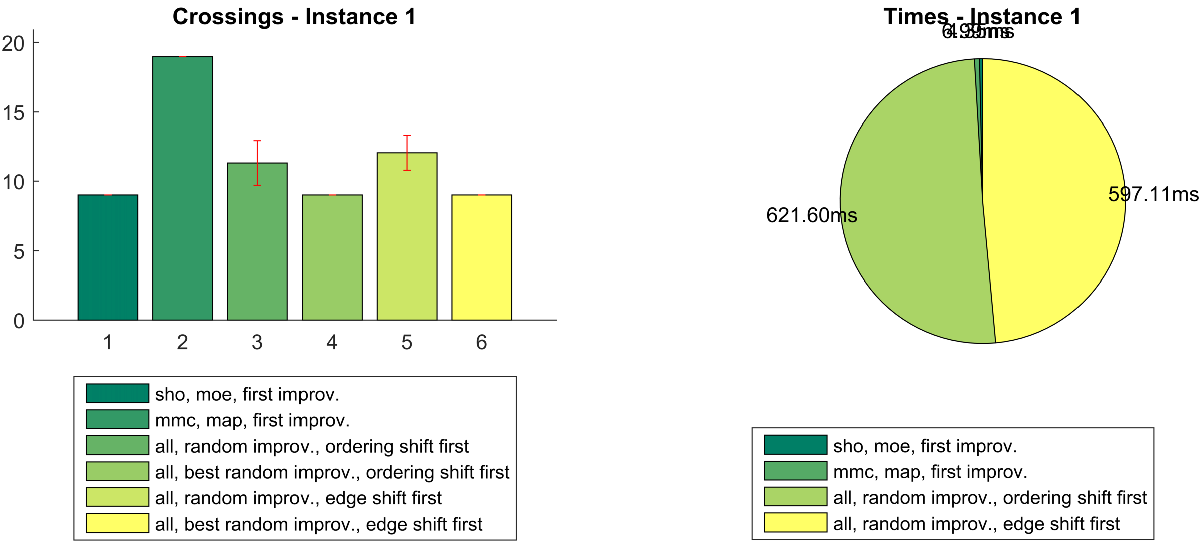
\includegraphics[width=0.8\textwidth]{instance1}
\end{figure}

\begin{figure}[h]
\centering
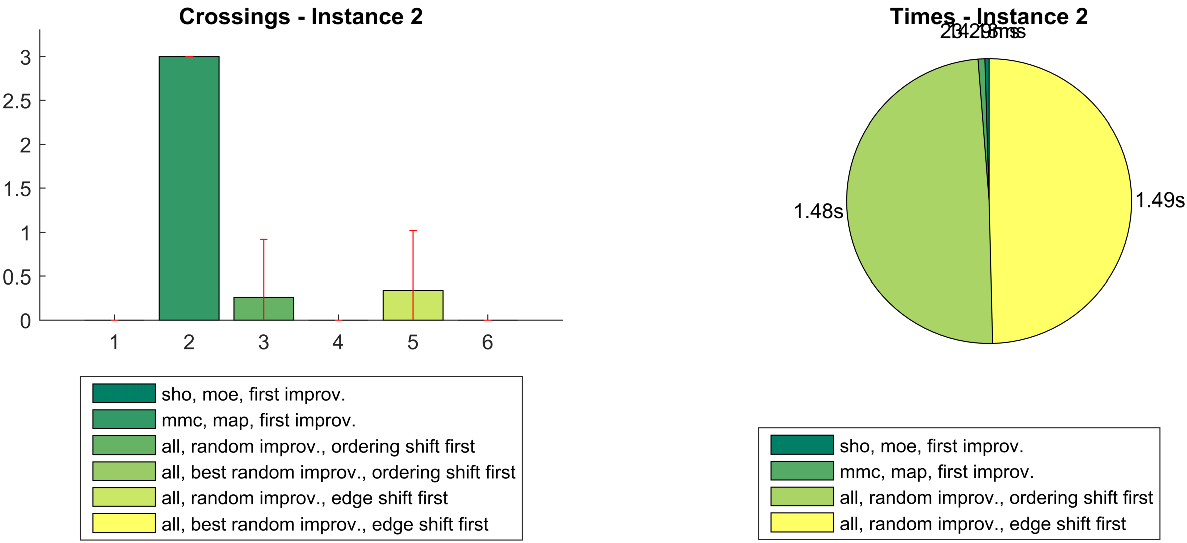
\includegraphics[width=0.8\textwidth]{instance2}
\end{figure}

\begin{figure}[h]
\centering
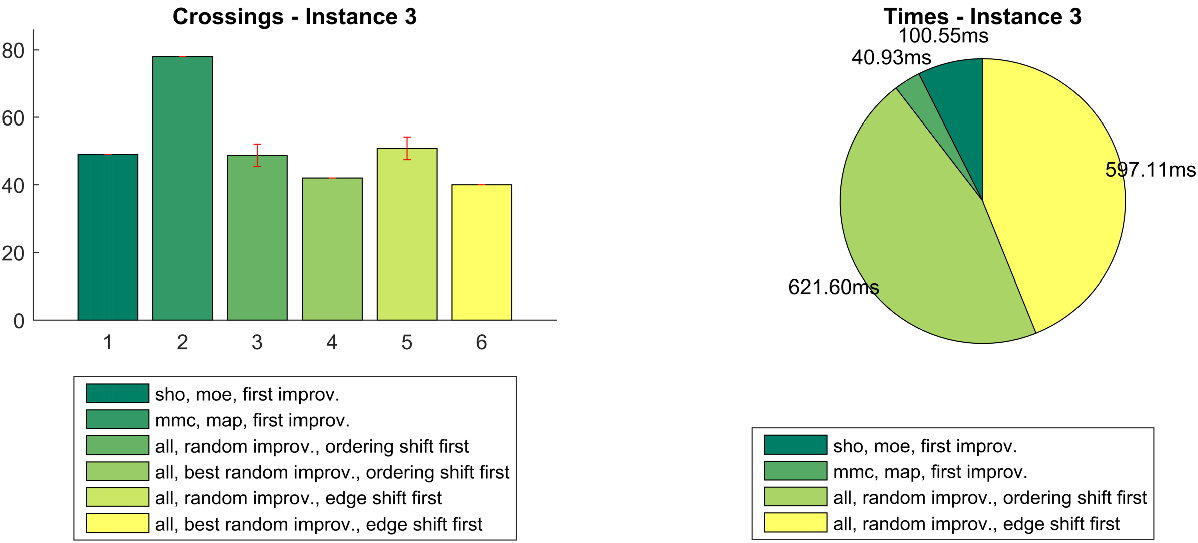
\includegraphics[width=0.8\textwidth]{instance3}
\end{figure}

\begin{figure}[h]
\centering
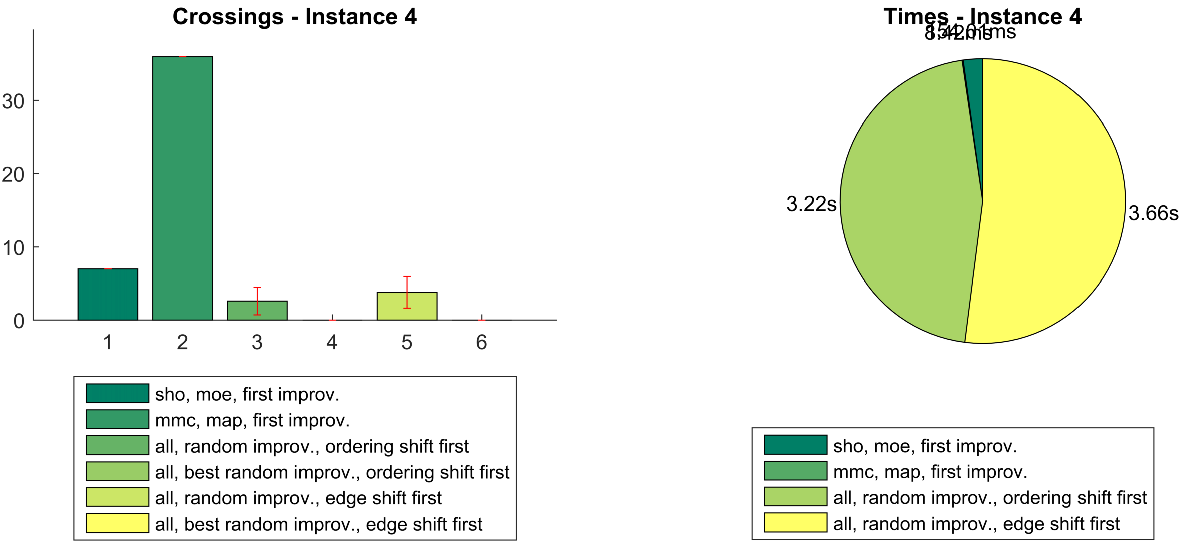
\includegraphics[width=0.8\textwidth]{instance4}
\end{figure}

\begin{figure}[h]
\centering
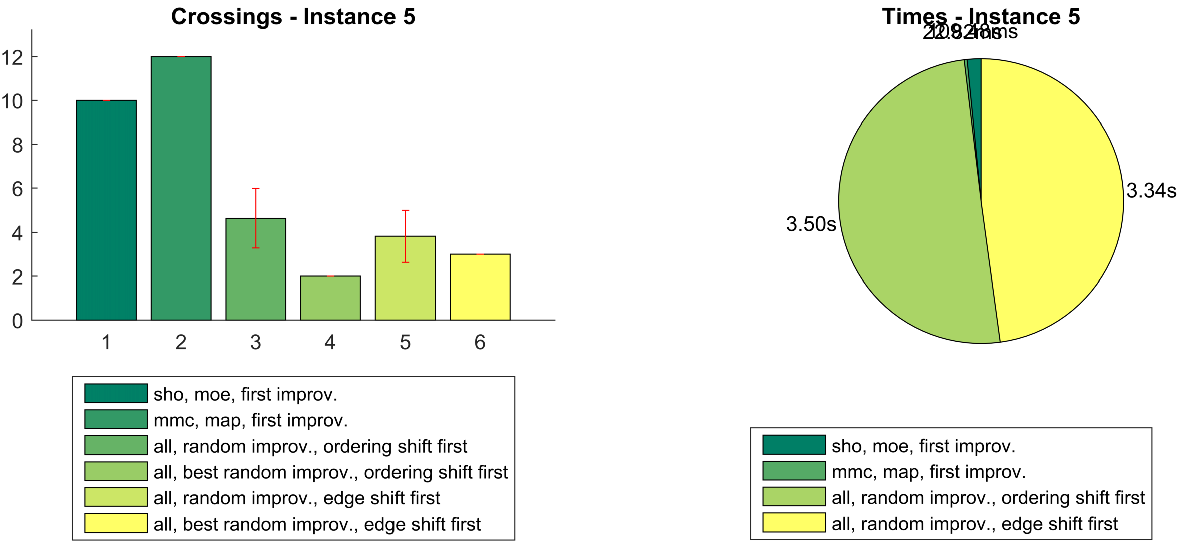
\includegraphics[width=0.8\textwidth]{instance5}
\end{figure}

\begin{figure}[h]
\centering
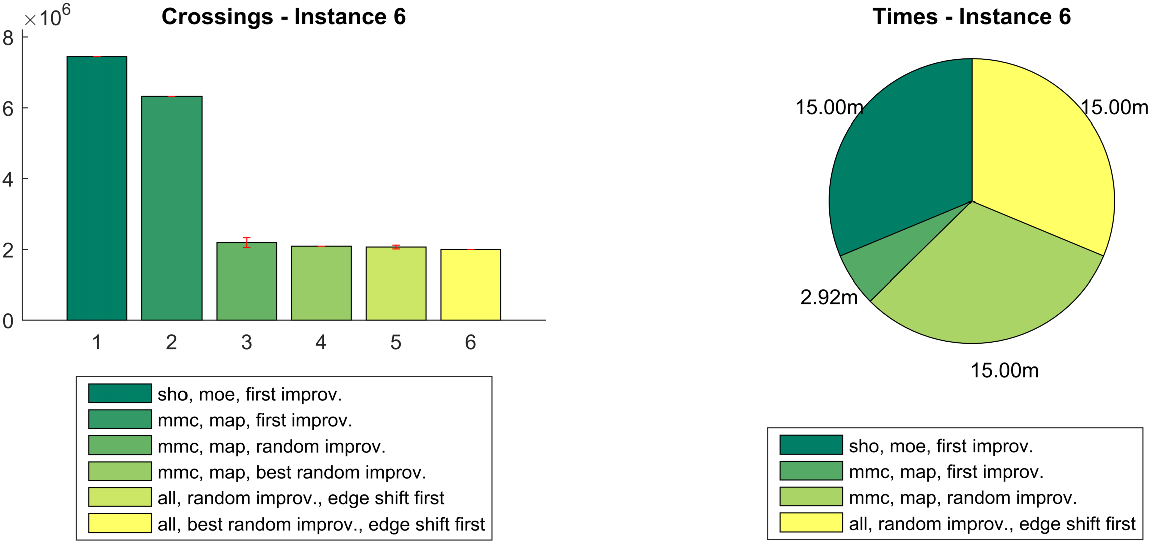
\includegraphics[width=0.8\textwidth]{instance6}
\end{figure}

\begin{figure}[h]
\centering
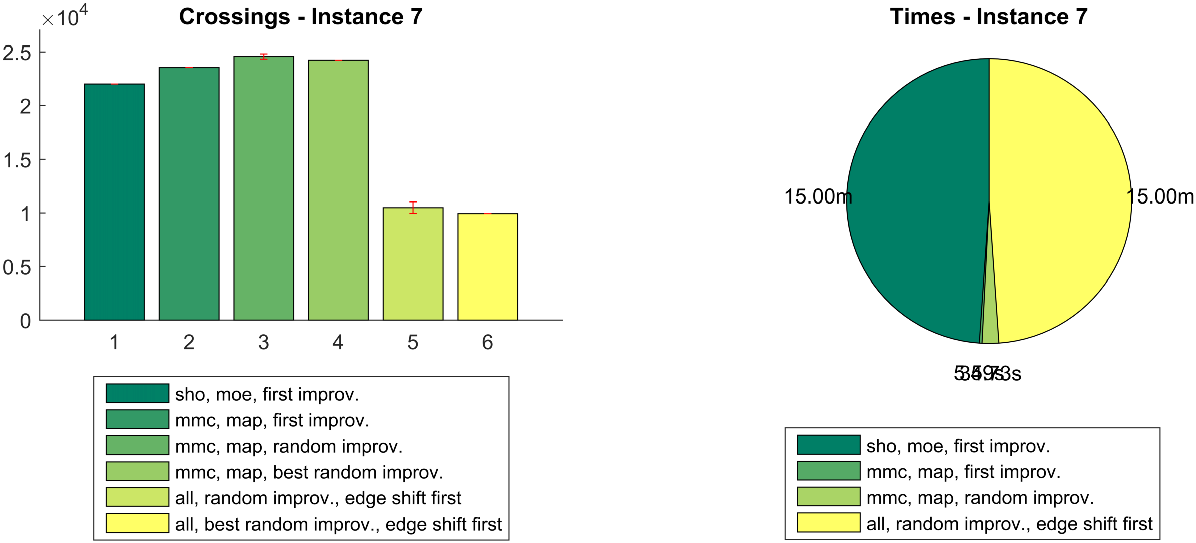
\includegraphics[width=0.8\textwidth]{instance7}
\end{figure}

\begin{figure}[h]
\centering
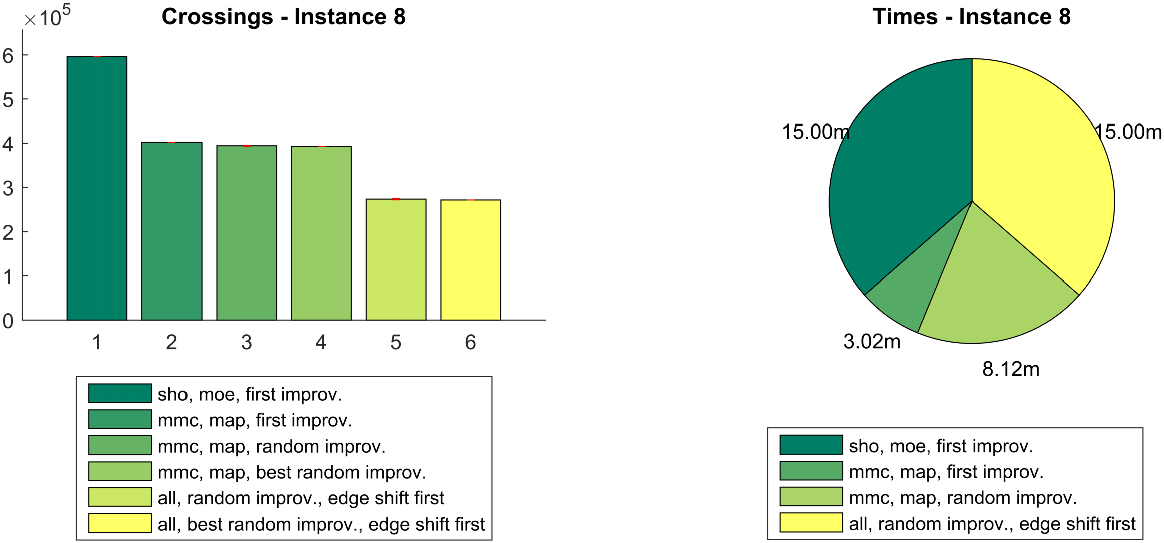
\includegraphics[width=0.8\textwidth]{instance8}
\end{figure}

\begin{figure}[h]
\centering
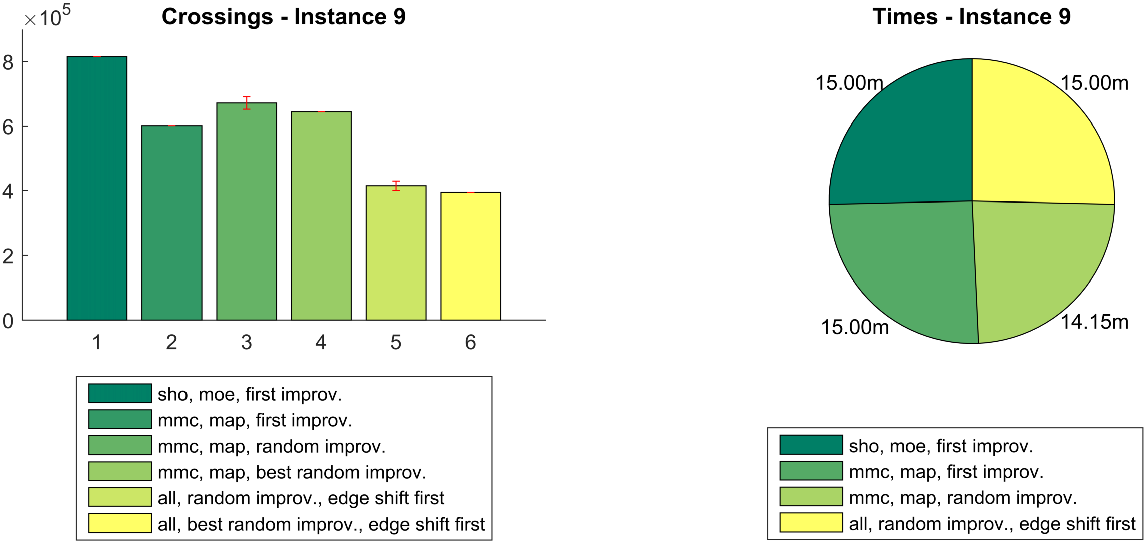
\includegraphics[width=0.8\textwidth]{instance9}
\end{figure}

\begin{figure}[h]
\centering
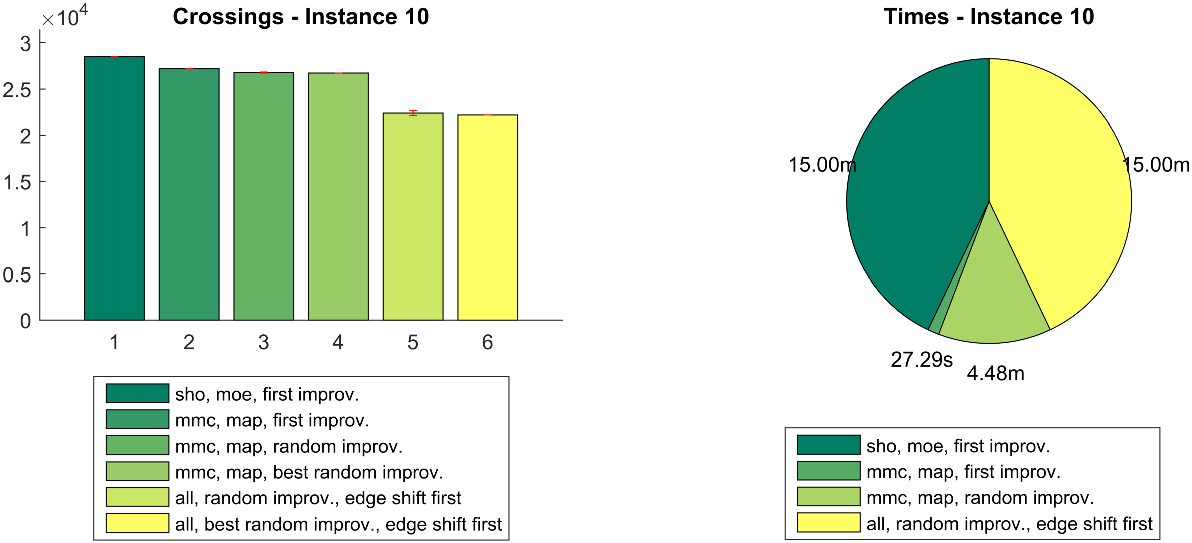
\includegraphics[width=0.8\textwidth]{instance10}
\end{figure}

\end{document}

